\section{Introduction}
\label{sec:introdction}

Video Large Language Models (VLLMs)~\cite{bai2025qwen2,zhu2025internvl3,zhang2023video,lin2023video,cheng2024videollama,li2024mvbench,weng2024longvlm,wu2023visual,wang2023chatvideo,li2023videochat,chen2024sharegpt4video} nowadays have showcased remarkable prominence for complex video understanding and comprehension. The visual encoder~\cite{zhai2023sigmoid,radford2021learning} converts sampled frames into video token sequences, which LLM then processes alongside text sequences to generate the responses. Increasingly demandings further require VLLMs to process longer and more complex video scenarios~\cite{li2024llama,chai2024auroracap,team2024gemini,weng2024longvlm}. 



Despite their effectiveness, the high computational cost and memory consumption of inference pose significant challenges, particularly making  inference computationally expensive when processing videos with numerous frames, which takes tens of thousands of input token count. Though some approaches~\cite{jin2024chat,maaz2023video,shen2024longvu,xu2024pllava,zohar2025apollo,song2024moviechat} perform trainable compression module to alleviate this issue, they still demand extensive training or fine-tuning, leading to high training costs. While prior works~\cite{yang2025visionzip,xing2024pyramiddrop,tao2025dycoke,bolya2022token,shang2025llava,zhang2024sparsevlm,shao2025holitom} have explored model compression and token pruning to mitigate the efficiency problem, achieving a desirable balance between efficiency and performance, but fail to exploit temporal dependencies across sampled frames.

\begin{figure}[t]
    % \vspace{0.5cm}
    \centering
    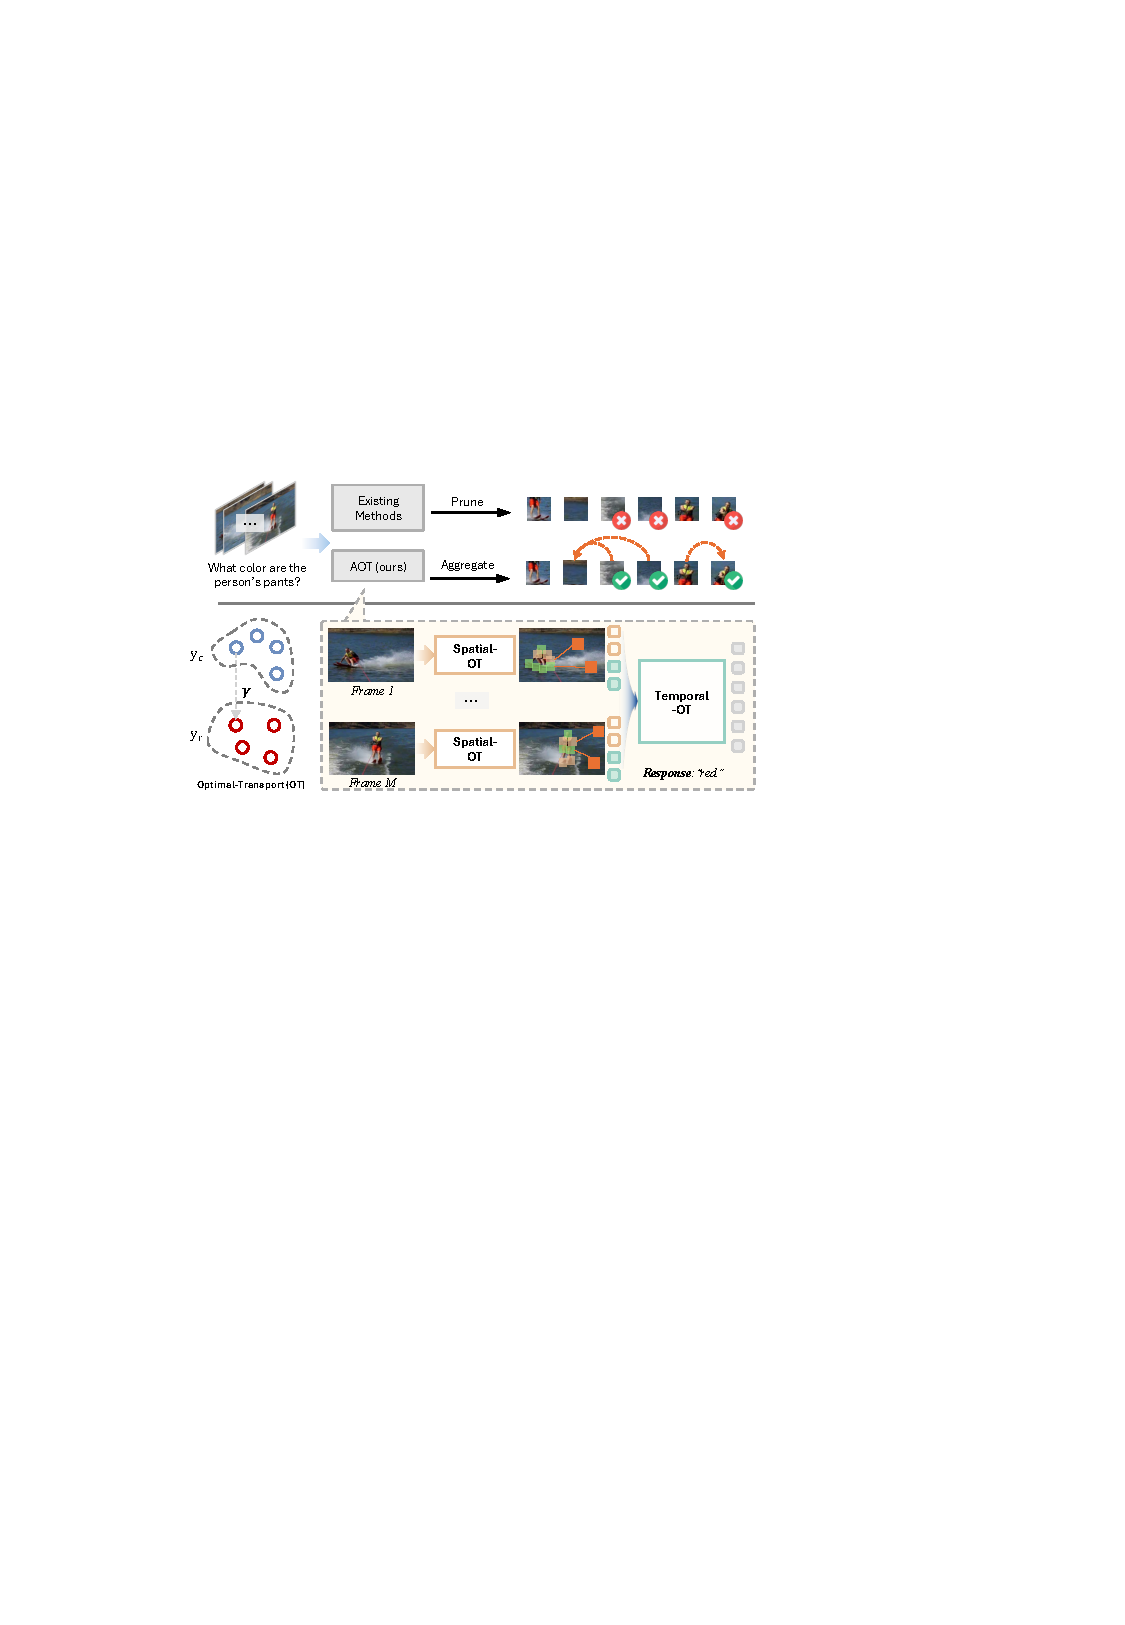
\includegraphics[width=\linewidth]{figs/cvpr2026_motivation.pdf}
    % \vspace{-0.6cm}
    \caption{The top is the essential differences compared with common token reduction methods, instead of simply removing unimportant or merging very similar tokens, ours utilizes a global optimization strategy to further exploit and aggregate necessary semantic and context from these onto the remaining tokens. Bottom is our proposed pipeline to adopt Optimal Transport to aggregate information within intra- and inter-frame levels for video tokens.}
    \label{fig:motivation_fig}
    \vspace{-0.2cm}
\end{figure}

Thus, developing effective methods to reduce video token redundancy while preserving critical semantical and contextual information is crucial for the widespread utility of video LLMs. Recently, video compression methods like DyCoke~\cite{tao2025dycoke} and PruneVid~\cite{huang2024prunevid} mainly prune at the LLM prefilling and decoding stages, processing video tokens analogous to textual tokens and ignoring specific characteristics of video. Moreover, some token pruning approaches~\cite{fu2024framefusion,bolya2022token,yang2025visionzip,shang2025llava} take the most-discriminative tokens while simply removing the low-discriminative or fusing many similar ones, vulnerable to token selection and neglecting informative regions or involving noisy backgrounds. A more video-specific pruning approach is necessary to fully exploit spatiotemporal redundancy while preserving appropriate visual contexts.



To alleviate this limitation, in this paper, we propose a new perspective that elaborates token \textit{\textbf{A}nchors} within intra-frame and inter-frame to comprehensively aggregate the semantic and context information via local-global \textit{\textbf{O}ptimal} \textit{\textbf{T}ransport} (\textbf{AOT}). Inspired by the AnyRes technique from MLLMs~\cite{li2024llava,chen2024far,zhang2024llavanextvideo}, we first perform a grid-wise local token selection to maintain the local prior while a global-level selection exclusive will be applied to select the global tokens with attention guidance, together serving as token \textit{anchors} for each frame. This strategy retains semantically important and spatially diverse token candidates.



Building on this insight, how to appropriately measure the relationship between the selected and unselected tokens remains a critical exploration, which aims to abstract necessary information. To address this, we introduce Optimal Transport (OT) to measure the distances between the selected token anchors and unselected tokens through a global optimization strategy. For intra-frame token pruning, we formulate token anchors and unselected tokens as the samplings of two discrete distributions and use OT to encourage fine-grained measurement matching (\textit{few-to-many}), while inverse cosine similarity among token sets serves as the cost matrix to be optimized. 
%
The distance calculation between token sets will be modeled as a discrete probability distribution where each token has an equal probability value based on optimal transport theory~\cite{villani2008optimal}.
Each token in the unselected set is a supplier who supplies a certain level of necessary contexts, and each token anchor is a demander who needs one unit of context. 
In this sense, each token anchor comprehensively consolidates the aggregation from unselected tokens globally under the optimized transport plan.



For inter-frame token pruning, we further utilize Optimal Transport to tackle temporal redundancy by establishing the first frame within each frame clip as the anchors, and then ensembling similar tokens across the consecutive frames and gradually updating the token anchors, while keeping dissimilar tokens to represent key temporal dynamics. This can be employed with uniform sampling or adaptive clustering frame clip.
After that, AOT leads to necessary local-global semantic and context aggregation across spatiotemporal dimensions by adopting Optimal Transport to assemble informative cues from numerous tokens under merging or removing. Differing from existing methods~\cite{tao2025dycoke,huang2024prunevid,liu2025hybrid,shen2024longvu}, our approach considers detailed intrinsic contributions of these tokens to compact token anchors shown in Fig.~\ref{fig:motivation_fig}, significantly accelerating Video LLM inference while preserving both temporal and visual integrity. After formulation, finding the best assignment solution is converted to solve an optimal transport plan, which can be quickly and efficiently solved by the off-the-shelf Sinkhorn-Knopp Iteration~\cite{cuturi2013sinkhorn} using GPU.



To evaluate the effectiveness of our method, we perform extensive experiments on  LLaVA-OneVision 7B and LLaVA-Video 7B models across MVBench~\cite{li2024mvbench}, LongVideoBench~\cite{wu2024longvideobench}, EgoSchema~\cite{mangalam2023egoschema}, and VideoMME~\cite{fu2025video}. Our approach reduces computational costs to just 8.3\% of the original FLOPs and prunes 90\% of video tokens while remarkably preserving 97.6\% of the original model’s performance across all benchmarks. These results clearly demonstrate the substantial practical advantages of our token reduction framework for efficient video LLM inference.
Our main contributions are:

\begin{itemize}
    \item To the best of our knowledge, we are the first to investigate how to aggregate subtle yet informative semantics and contexts from merging or removing tokens into remaining tokens, instead of simply merging or removing.
    
    \item We study how to first facilitate token anchors that consider both local and global prior, leading to semantically important and spatially diverse candidates.
    
    \item We explore Optimal Transport to aggregate spatiotemporal context from the transport plan within intra- and inter-frame to preserve temporal and visual fidelity with a training-free pipeline.

    \item We evaluate our method in a wide spectrum of video benchmarks and present competitive performances under constrained token budgets.
\end{itemize}

